%Dokumentinnstillinger:---------------------------------
%Ved å google flitting kan du finne ut hva de forskjellige tingene her betyr, og hvordan du kan gjøre eventuelle endringer.
\documentclass[a4paper,11pt,norsk]{article}
\usepackage[utf8]{inputenc}
\usepackage{a4wide}
\usepackage{lmodern}
\usepackage[T1]{fontenc}
\usepackage{babel}

\setlength{\parindent}{0pt} 
\setlength{\parskip}{2ex}
\usepackage{fixltx2e}
\usepackage{amsmath}
\usepackage[pdftex, pdfborderstyle={/S/U/W 0}]{hyperref}
\usepackage{graphicx}
\usepackage[font=small,labelfont=bf]{caption}
\usepackage{tabularx}
\usepackage{multirow}
\usepackage{circuitikz}
\usepackage{pst-node,pst-circ}
% Adds seperation between two elements with a comma. Format: "    ,    ".
\newcommand{\comma}{\quad , \quad}
% Gives double underline under selected text.
\def\dunderline#1{\underline{\underline{#1}}}
% Faster way to make an equation that can be formatted with "&" to look nice.
\def\spliteq#1{\begin{equation}\begin{split}{#1}\end{split}\end{equation}\\}
%------------------------------------- End -------------------------------------

\begin{document}

%Headingdel:---------------------------------------------
\begin{minipage}[c]{0.15\textwidth}
\includegraphics[width=2.0cm]{elsys_pos_staaende_ntnu.png}
\end{minipage}
\begin{minipage}[c]{0.85\textwidth}

\renewcommand{\arraystretch}{1.7}
\large 
\begin{tabularx}{\textwidth}{|X|X|}
\hline
\multicolumn{2}{|l|}{} \\
\multicolumn{2}{|l|}{\huge \textbf{Designnotat 6}} \\
\multicolumn{2}{|l|}{}  \\
\hline
\multicolumn{2}{|l|}{Tittel: 
%Skriv inn tittel her:------------------------------------------
Ulineær Oscillator
} \\
\hline
\multicolumn{2}{|l|}{Forfattere: 
%Skriv inn forfattere her:--------------------------------------
Sindre Danielsen
} \\
\hline
%Skriv inn versjon og dato her her:-----------------------------
Versjon: 1.5 & Dato: 11.12.21
\\
\hline 
\end{tabularx}
\end{minipage}
\normalsize

%Automatisk generert innholdsfortegnelse:------------------

\setlength{\parskip}{0ex}
\renewcommand{\baselinestretch}{0.1}\normalsize
\tableofcontents
\renewcommand{\baselinestretch}{1.00}\normalsize
\setlength{\parskip}{2ex}
\rule{\textwidth}{1pt}

%Selve rapporten:----------------------------------------÷
\newpage
\section{Problembeskrivelse}
\label{sec:innledning}
For å generere et signal ved en spesifisert frekvens, så brukes en oscillator. En oscillator har kun tilgang til en DC-strøm/spenning og fra det, så generes et signal på den formen som er ønsket for formålet. Vi skal her analysere en mulig løsning, kalt en ulineær oscillator. Hensikten bak denne er å generere et sinussignal gjennom ulineær oppførsel, som hele tiden forsøker å holde dempningsfaktoren $\zeta = 1$ (for mer om dempning, se \cite{dampning}). En slik oscillator er vist ved figur~\ref{fig: oscillator generalisert}.
\\
\begin{figure}[htbp]
    \centering
    \begin{circuitikz} [american voltages, european resistors, baseline=(current bounding box.center)]
        \ctikzset { label/align = straight }
        \draw (0,0)
        % Left dashed box
        node[draw,solid,minimum width=2cm,minimum height=1cm,anchor=south west] at (0,2) {$\mathbf{g(\cdot)}$}
        ++ (0, 0.5)
        -- ++ (-1,0)
        to[short] ++ (0, 2)
        -- ++ (1, 0)
        % Right dashed box
        node[draw,solid,minimum width=2cm,minimum height=1cm,anchor=south west] at (0,0) {$\mathbf{H}$}
        ++ (2, 0)
        -- ++ (1, 0)
        to[short, -*] ++ (0, -2)
        -- ++ (-1,0)
        -- ++ (2,0)
        % y(t)
        ;
        % g(*) arrow
        \draw[-Triangle] (2+1, 0.5 + 2) -- ++ (-1,0);
        % H arrow
        \draw[-Triangle] (-1, 0.5) -- ++ (1,0);
        % y(t) arrow
        \draw[-Triangle] (2, 0.5) -- ++ (2,0);
        \node[] at (4.5,0.5) {$y(t)$};
        
    \end{circuitikz}
    \caption{Oppførsel til en ulineær oscillator.}
  \label{fig: oscillator generalisert}
\end{figure}
\\
Den ulineære oppførselen skapes av $g(\cdot)$, mens $H$ er et båndpassfilter som gir ut en ønsket \\ frekvens på utgangssignalet $y(t)$.
\\\\
For et slikt system, så er det verdt å vurdere sammenhengen mellom teorietiske verdier og verdier som realiseres. For oscillatorer er det hensiktsmessig å se på kvaliteten til $y(t)$. Det blir ofte oppgitt på formen \textit{SNR} (Signal-To-Noise-Ratio).


\newpage

\section{Prinsipiell løsning}
\label{sec:prinsipielllosning}
Kretsdesignet for den oscillatoren som skal undersøkes er vist ved figur~\ref{fig: oscillator kretsdesign}.
\\
\begin{figure}[htbp]
    \centering
    \begin{circuitikz} [american voltages, european resistors, european vresistors, baseline=(current bounding box.center)]
        \ctikzset { label/align = straight, diodes/fill=black}
        
        \draw (0,0)
        (2.70,-0.490) node[op amp] (opamp1) {}
        % Creates first op amp
        (opamp1.up) ++ (0,0.5)  (opamp1.up)
        (opamp1.down) ++ (0,-0.5)
        (opamp1.+) node[ground] ++ (0, -1.5)
        (opamp1.-) to[short,-*] ++ (-0.5, 0)
        
        % Upper diode
        -- ++ (0, 2)
        -- ++ (0.75, 0)
        -- ++ (0, 0.5)
        to[diode] ++ (2,0)
        -- ++ (0, -0.5)
        
        % Bottom diode
        (opamp1.-) ++ (0.25, 2)
        -- ++ (0, -0.5)
        to[diode, invert] ++ (2, 0)
        -- ++ (0, 0.5)
        
        % Resistor parallell to diodes
        (opamp1.-) ++ (-0.5, 2) -- ++ (0, 1.5)
        to[R=$R$] ++ (3.38, 0)
        -- ++ (0, -1.5)
        
        % Into first opamp
        (opamp1.-) ++ (-0.5, 0) to[R=$R_1$] ++ (-2.5,0)
        
        % Out of first opamp
            % Finishing the diode connection
            (opamp1.out) ++ (0.5, 0) -- ++ (0, 2.5)
            -- ++ (-0.625,0)
            
        (opamp1.out) to[short, -*] ++ (0.5, 0)
        to[R=$R_2$] ++ (2.5, 0)
        
        % Creates second opamp
        ++ (1.75, -0.49) node[op amp] (opamp2) {}
        (opamp2.up) ++ (0,0.5)  (opamp.up)
        (opamp2.down) ++ (0,-0.5)
        (opamp2.+) node[ground] ++ (0, -1.5)
        (opamp2.-) to[short,-*] ++ (-0.5, 0)
        
        % To resistor across opamp2
        -- ++ (0, 2)
        to[R = $R_f$] ++ (3.375,0)
        -- ++ (0, -2.525)
        
        % Opamp2 out
        (opamp2.out) to[short, -*] ++ (0.5, 0) 
        to[L=$L$] ++ (0, -2)
        to[C=$C$] ++ (0, -1)
        to[short, -*] ++ (0, -1)
        -- ++ (-11.82, 0)
        -- ++ (0, 4.98)
        
        % y(x) outsignal
        (opamp2.out) ++ (0.5, -4)
        to[short, -o] ++ (2, 0)
        ++ (0.75, 0) node[] {$y(x)$}
        
        % Resistor in RCL:
        (opamp2.out) ++ (0.5, -4)
        to[R=$R_H$] ++ (0,-2)
        node[ground] ++ (0, -0.5)
        
        % RCL filter:
        node[draw,dashed,minimum width=2.5cm,minimum height=6.6cm,anchor=south west] at (9.10,-8) {}
        node[] at (10.35, -8.5) {Båndpass-filter}
        ;
        
    \end{circuitikz}
    \caption{Kretsdesignet til en ulineær oscillator.}
    \label{fig: oscillator kretsdesign}
\end{figure} \\
Her er $R_1$ en inngangsmotstand til den første opampen og $R_2$ til den andre opampen. Mostanden $R$ fungerer som en tilbakekobling, som er i parallell med to omvendt koblede dioder i parallell. Motstanden $R_f$ er tilbakekoblingen for den andre opampen. Motstandene fungerer i hovedssak til å bestemme forsterkningen på opampene. Det forklares i seksjon~\ref{sec: opamp}. For å filtrere ut signalet består systemet av et båndpassfilter med spolen $L$, kondensatoren $C$ og båndbredde-motstanden $R_H$.
\newpage
\subsection{Ulineær analyse}
Kretsen i figur~\ref{fig: oscillator kretsdesign} har en ulineær oppførsel på grunn av diodene, som blir brukt. Generelt sett, så vil en lineær oscillator ha en differensiallikning på formen 
\\
\begin{equation}
    \ddot{y} + (1 + G) \frac{R}{L}\dot{y} + \frac{1}{LC}y = 0 \: .
\end{equation}
\\
$G$ er forsterkningsfaktoren til opampenene. Denne har kun teoretisk interesse, siden å ha en $G$ alltid lik 1 er ikke mulig i praksis. Derfor brukes dioder for å utvikle et en oppførsel som vil rette seg inn mot $G = 1$, for hver gang $G$ øker eller minker. For en mer teoretisk gjennomgåelse, se \cite{Oscillator bb}. \\\\ Et at problemene med ulineær oppførsel er at det blir fort komplisert å løse en differensiallikning beskrevet ved 
\begin{equation}
    \ddot{y} + \left[ \dot{y} - \frac{d}{dt} g(y)  \right] + \frac{1}{LC}y \: .
\end{equation}
\\\\
Fremfor å gå frem matematisk, så kan vi bruke det vi allerede vet om dioder. Det er en matematisk modell for dioder, kalt den \textit{eksponentielle diodemodellen} \cite{diode modell}. Likningen er gitt ved 
\begin{equation}
    i_D = I_0 \left( e^\frac{v}{V_0} - 1 \right) \: .
\end{equation}
\\

Den ulineære delen av kretsen er vist ved figur~\ref{fig: ulineær kretsdel} med de viktige analytiske strømmene oppsatt. \\
\begin{figure}[htbp]
    \centering
    \begin{circuitikz} [american voltages, european resistors, european vresistors, baseline=(current bounding box.center)]
        \ctikzset { label/align = straight, diodes/fill=black}
        
        \draw (0,0)
        to[short, i= $i$, *-] ++ (1, 0)
        -- ++ (1,0)
        % Lower diode
        -- ++ (0, -1)
        to[diode] ++ (2,0)
        -- ++ (0,1)
        % Upper diode
        (0,0) ++ (2,0)
        -- ++ (0, 1)
        to[diode, invert] ++ (2, 0)
        -- ++ (0, -1)
        to[short, i=$i_D$] ++ (1,0)
        to[short, -*] ++ (1,0)
        node[] at (-0.3,0) {$v$}
        
        % Resistor parallell to diodes
        (0,0) ++ (1, 0) to[short, i=$i_R$] ++ (0, 3)
        to[R=$R$] ++ (4, 0)
        -- ++ (0, -3)
    \end{circuitikz}
    \caption{Ulineært kretssystem.}
    \label{fig: ulineær kretsdel}
\end{figure} \\
\newpage

Strømmen finner vi ved strømdelingen 
\begin{equation}
    i = i_D + i_R = i_D + \frac{v}{R} \: .
\end{equation}
\\
Spenninga i paralellkoblinga er da gitt ved 
\begin{equation}
    v = V_0 ln\left(1 + \frac{i_D}{I_0} \right).
\end{equation}

Vi vet for dioder at for små spenninger, som varierer litt avhengig av dioden, så går det neglisjerbar mengde strøm. Det betyr at kretsen kun oppfører seg som en motstand $R$.
Når strømmen $i$ er stor, så vil diodene dominere strømmen, slik at vi får en oppførsel vist ved figur~\ref{fig: diode kurve}. 
\begin{figure}[htbp]
    \centering
    \includegraphics[width=0.5\textwidth]{img/Diode_Curve.png}
    \caption{Kurven for diodeoppførselen $i(v)$.}
    \label{fig: diode kurve}
\end{figure}\\

\newpage
Det ulineære systemet i figur~\ref{fig: ulineær kretsdel} vil utvikle en invers funksjon av kurven $i(v)$ kalt $f(i)$ fra figur~\ref{fig: f(i) kurve}. Egenskapen til $f(i)$ er at den vil hele tiden forsøke å inrette spenningen slik at den blir lineær. Det vil si at dersom spenningen blir for høy, så vil den forsøke å minke spenningen. Når spenningen blir for lav, så vil den forsøke å øke spenningen. En grafisk forestilling er vist av grensesyklusen i figur~\ref{fig: fasediagram}.
\begin{figure}[htbp]
    \centering
    \includegraphics[width=0.5\textwidth]{img/f_i diode kurve.png}
    \caption{Oppførselen $f(i)$ til det ulineære systemet i figur~\ref{fig: ulineær kretsdel}.}
    \label{fig: f(i) kurve}
\end{figure}\\

\begin{figure}[!htbp]
    \centering
    \includegraphics[width=0.5\textwidth]{img/Grensesyklus.png}
    \caption{Grensesyklus: Ettersom forsterkninga minker/øker så rettes den inn mot en stabil sirkel.}
    \label{fig: fasediagram}
\end{figure} \\



\subsection{Opampenes funksjonalitet}\label{sec: opamp}
Kretsen tar i bruk to opamper med ulik tilbakekobling.
Den første har et ulineært system, mens opamp 2 ser ut til å være kun en forsterker med en bufferegenskap. 
Det kan også merkes at det er valgt å bruke inverterende oppkobling på opampene, som kan forhindre ustabiltet i signalet enn dersom man bruker ikke-inverterende. Det er da hensiktsmessig å invertere signalet to ganger, dersom fasen på signalet er av betydning. 
\\
For opamp 2, så har vi en den generelle likningen for den inverterte forsterkningen 
\begin{equation}
    A_v = -\frac{v_o}{v_i} = -\frac{R_o}{R_i}.
\end{equation}
Og dersom den brukes som en buffer, så har vi at 
\begin{equation}
    A_v = -\frac{R_1}{R} = -\frac{R_F}{R_2} = -1\cdot y(x) \:.
\end{equation}

\newpage


\newpage
\subsection{Bestemme frekvensen på $y(t)$}
Båndbreddens senterpunkt på $y(t)$ for en RCL krets er gitt ved frekvensen
\begin{equation}\label{eq: f_0}
    f_0 = \frac{1}{2\pi \sqrt{LC}} \:.
\end{equation}
Størrelsen på $R_H$ bestemmer bredden på båndpasset, samt hvor mye ampltiuderesponsen minker. Når impedansen $Z$ øker så vil amplituderesponsen minke. Frekvensen er gitt ved $\omega = 2\pi f$. Slik at vi får en impedans gitt ved
\begin{equation}
    Z = \frac{1}{j\omega C} + j\omega L + R_H.
\end{equation}
Den reelle motstandsverdien for $\omega$ er gitt ved $|Z|$.

\newpage
\section{Realisering og test}
\label{sec:realisering}
En teoretisk frekvens $f_0 = 2750$Hz. velges for å teste systemet. \\
Oppkoblingen av kretsen bruker da komponentverdiene gitt ved tabell~\ref{table: reelle verdier}.
\begin{table}[htbp]
\centering
\begin{tabular}{ |c|c|c|c| } 
\hline
\textbf{Navn} & \textbf{Verdi} & \textbf{Beskrivelse}\\
\hline
$L$ & $179$mH & Valgt pga. tilgjengelighet. \\
\hline
$C$ & $20$nF & Bedre å gå litt for stort enn for smått.
\\
\hline
$R$ & $\in[0, 9]$k$\Omega$ & Potensiometer.
\\
\hline
$R_1$ & $0.97$k$\Omega$ & 
\\
\hline
$R_2$ & $9.86$k$\Omega$ & 
\\
\hline
$R_f$ & $9.86$k$\Omega$ & 
\\
\hline
$R_H$ & $18.7$k$\Omega$ & 
\\
\hline
Dioder & 1N4007 & Tilgjengelige dioder.
\\
\hline
opamp & LF353N & Tilgjengelige opamper.
\\
\hline
\end{tabular}
\caption{Reelle verdier på komponentene basert på tabell~\ref{table: teoretiske verdier}.}
\label{table: reelle verdier}
\end{table}
\\




\begin{table}[htbp]
\centering
\begin{tabular}{ |c|c|c|c| } 
\hline
\textbf{Navn} & \textbf{Verdi} & \textbf{Beskrivelse}\\
\hline
$L$ & $179$mH & Målt verdi av spole. \\
\hline
$C$ & $18.7$nF & Likning~\ref{eq: C}.
\\
\hline
$R_1$ & $1$k$\Omega$ & Vanlig verdi på inngangsmotstand.
\\
\hline
$R_2$ & $10$k$\Omega$ & Valgt verdi.
\\
\hline
$R_f$ & $10$k$\Omega$ & $R_f = R_2 \implies$ buffer.
\\
\hline
$R_H$ & $20$k$\Omega$ & for å minke båndbredden.
\\
\hline
\end{tabular}
\caption{De teoretiske verdiene av komponentene i figur~\ref{fig: oscillator kretsdesign}. }
\label{table: teoretiske verdier}
\end{table}
\\
Ved oppkobling av en krets som har spoler og kondensatorer, så er det ofte lurt å bestemme seg for en spole og dermed finne kondensator verdien.
Målte en tilgjengelig spole $L = 179$mH og omformer så likning~\ref{eq: f_0}, slik at  \\
\begin{equation} \label{eq: C}
    C = \frac{1}{L(2\pi f_0)^2} = 18.7\textrm{nF} \: .
\end{equation} \\
\\
\newpage
For å lettere evaluere hva som foregår i den ulineære delen av kretsen, så brukes et potensiometer for $R$. Måler to verdier for $R$ i et oscilloskop. Det gir resultatene: \\
\begin{itemize}
    \item $R = 3.96$k$\Omega \implies y(t)$ og spolesignalet $v_L(t)$ i figur~\ref{fig: oscilloskop størst SNR} og fasediagrammet i figur~\ref{fig: fasediagram størst SNR}.
    \item $R = 1.3$k$\Omega \implies y(t)$ og $v_L(t)$ i figur~\ref{fig: oscilloskop lavest SNR} og fasediagrammet i figur~\ref{fig: fasediagram lavest SNR}.
\end{itemize} \\
\begin{figure}[htbp]
    \centering
    \includegraphics[width=1.0\textwidth]{img/os_R_3_96.png}
    \caption{Signalene $y(t)$ og $v_L(t)$ for $R = 3.96$k$\Omega$.}
    \label{fig: oscilloskop størst SNR}
\end{figure}
\newpage

\begin{figure}[htbp]
    \centering
    \includegraphics[width=1.0\textwidth]{img/fdg_R_3_96.png}
    \caption{Fasediagrammet til $y(t)$ mot $v_L(t)$ for $R = 3.96$k$\Omega$.}
    \label{fig: fasediagram størst SNR}
\end{figure}\newpage

\begin{figure}[htbp]
    \centering
    \includegraphics[width=1.0\textwidth]{img/os_R_1_3.png}
    \caption{Signalene $y(t)$ og $v_L(t)$ for $R = 1.3$k$\Omega$.}
    \label{fig: oscilloskop lavest SNR}
\end{figure}\newpage

\begin{figure}[htbp]
    \centering
    \includegraphics[width=1.0\textwidth]{img/fdg_R_1_3.png}
    \caption{Fasediagrammet til $y(t)$ mot $v_L(t)$ for $R = 1.3$k$\Omega$.}
    \label{fig: fasediagram lavest SNR}
\end{figure}\newpage

Vi kan sammenlikne dataene fra fasediagrammene og signalresponsene med den målte SNR fra et oscilloskop. \\\\
Ved $R \approx 3.96$k$\Omega$, så minker stigningen av SNR betraktelig. Velger derfor å stoppe her. Det som skjer når vi øker $R$ er at målingen over spolen blir mindre og mindre sinusformet, slik at fasediagrammet ikke blir sirkulært, men får et par områder (topp- og bunn-punktet til spolen) som spriker ut fra sirkelen.
Målingen ved bruk av oscilloskop gir en SNR $\approx 17.1$dB.
\\\\
Ved $R \approx 1.3$k$\Omega$, så er fasediagrammet tilnærmet sirkulært (dersom man skalerer x-aksen litt). Derimot så er SNR$=14.91$dB, som er betrakelig mindre enn for $R = 3.96$k$\Omega$. \\
Her kan vi observere at $v_L$ er tilnærmet proporsjonal med $y(t)$ (har en faseforskyvning).
\\\\
Ved testing, så viser det seg at ved å øke $R$ fra $3.96$k$\Omega$ til $9$k$\Omega$, så får SNR ikke noe betydelig vekst, men fasediagrammet forvrenges mer.
\\\\
For den realiserte frekvensen av $f_0$, så har den et avvik. Den reelle frekvensen blir $2440$Hz. En del av årsaken til avviket er på grunn av avviket i kondensatorverdien fra teoretisk til realisering. Avvik i frekvens kan også forekomme på grunn av ulineær oppførsel.
\newpage

\begin{figure}[htbp]
    \centering
    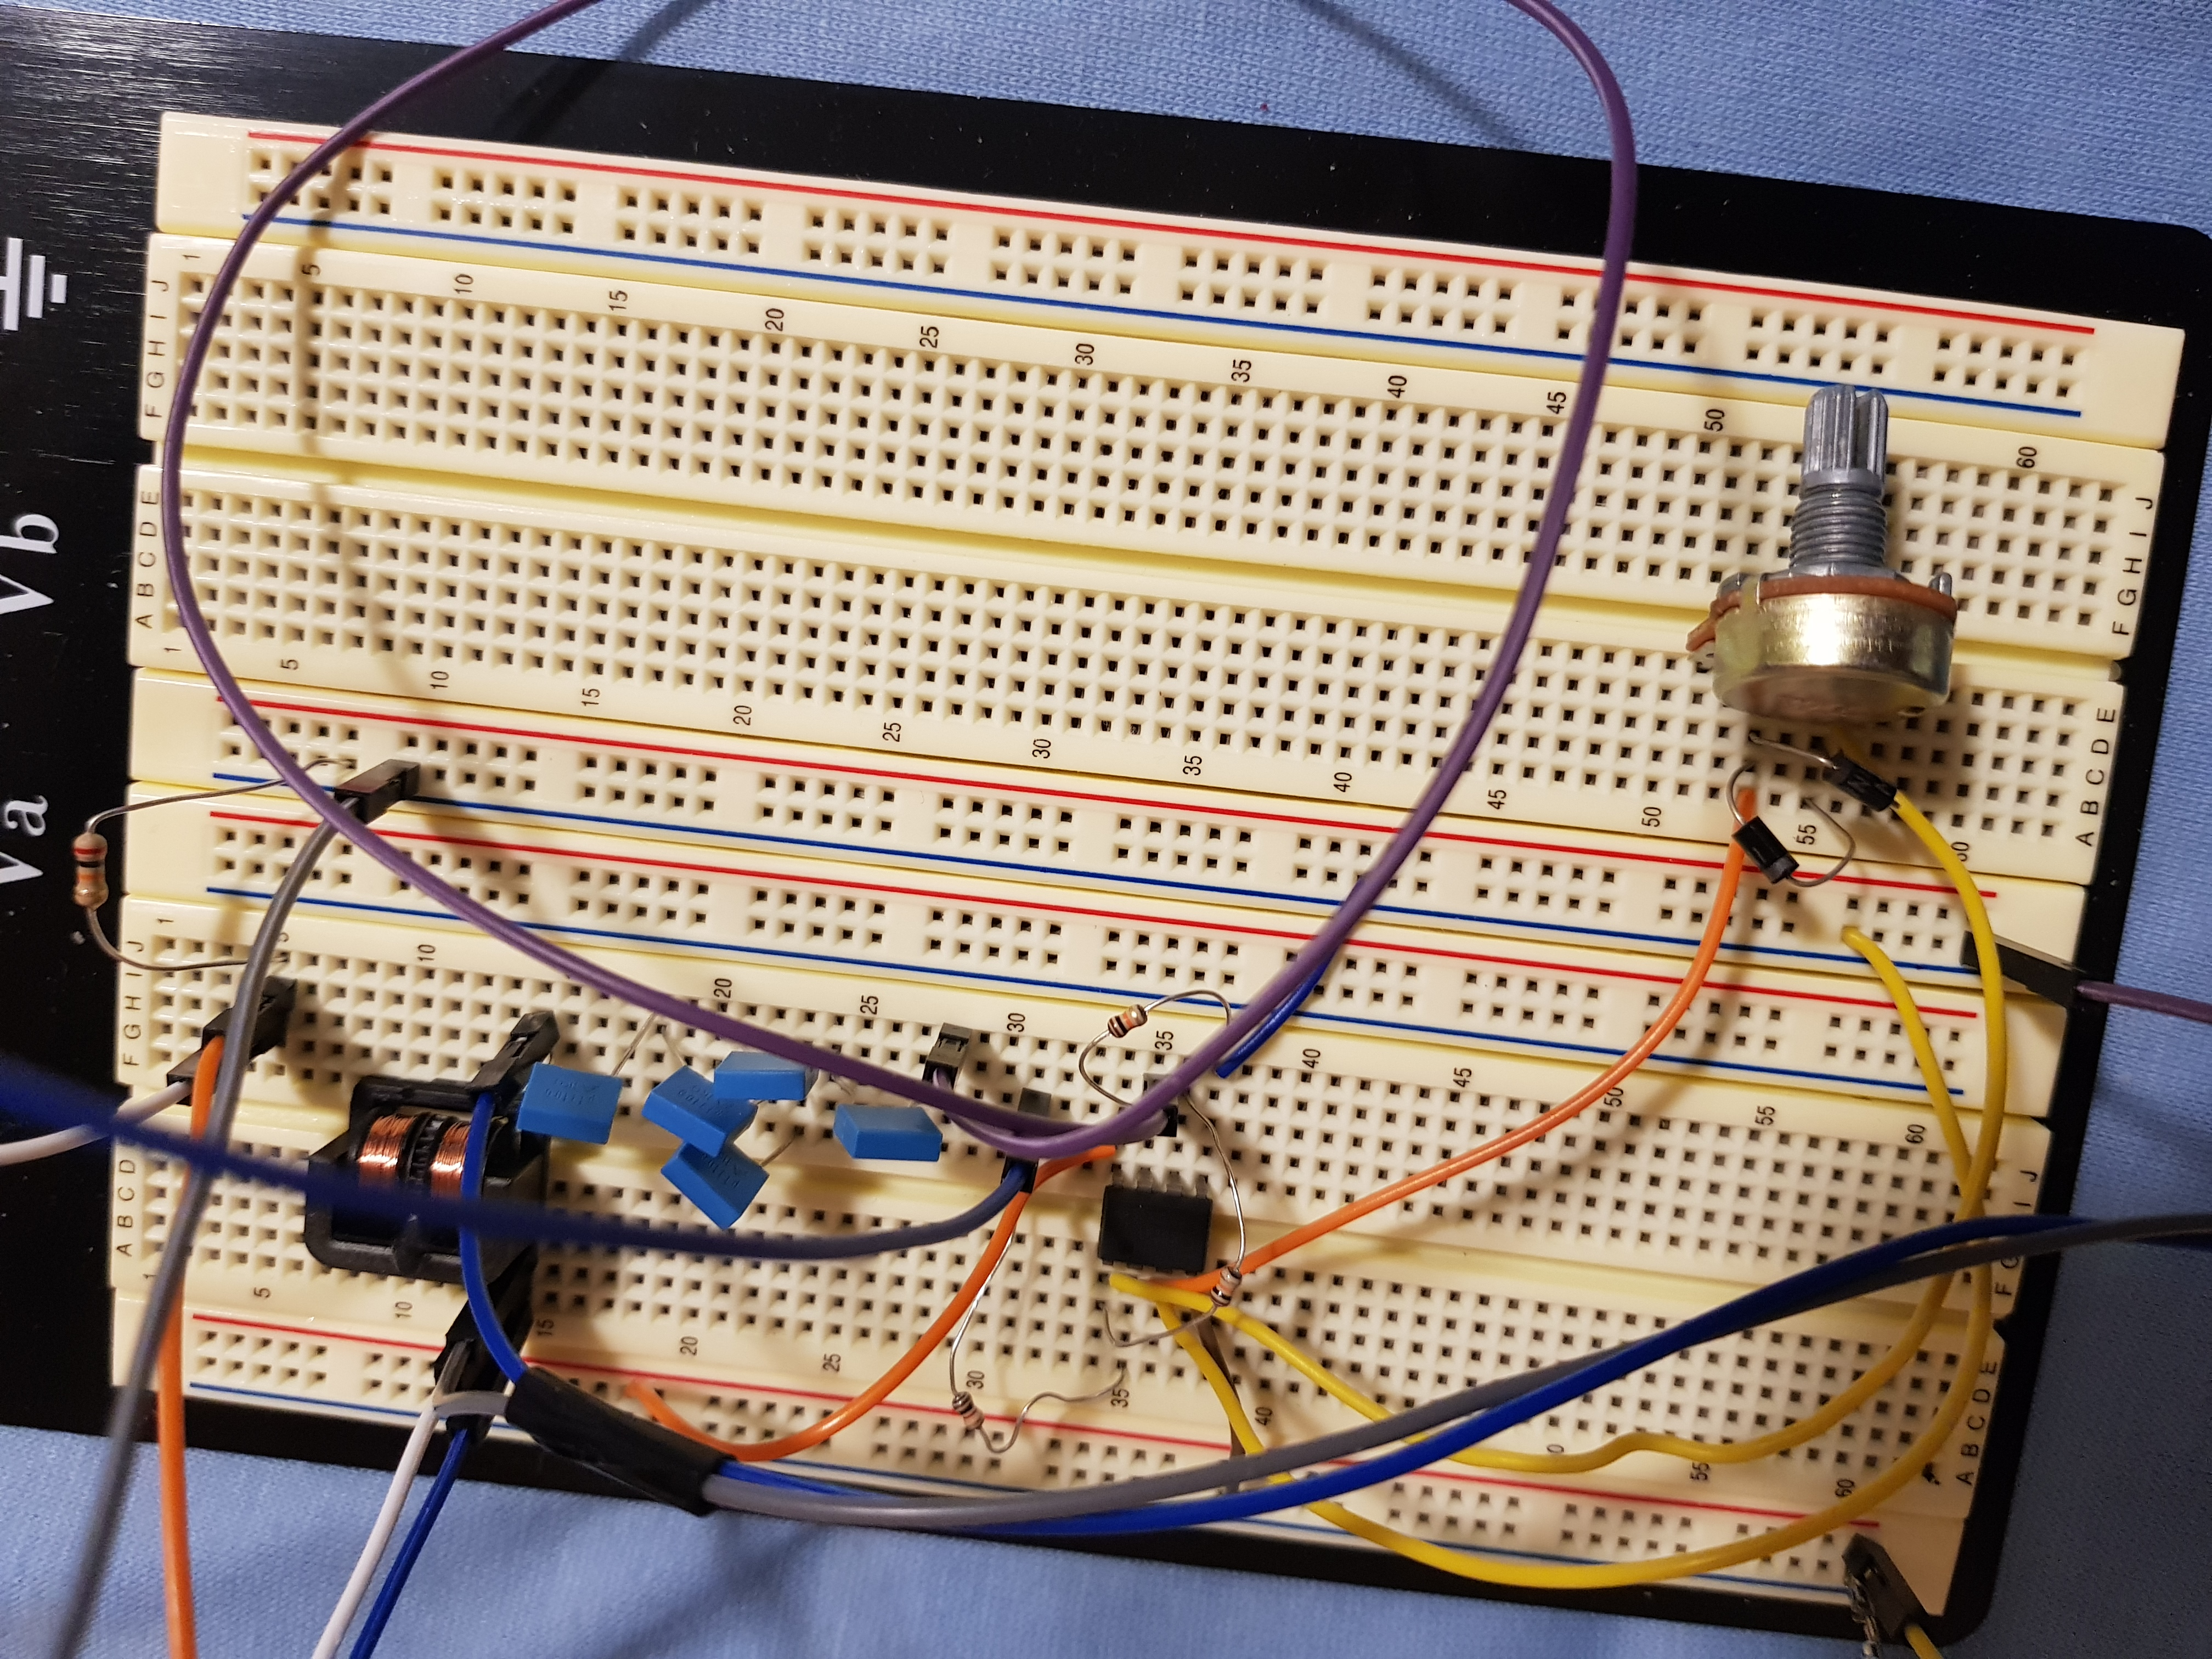
\includegraphics[width=0.8\textwidth]{img/real.jpg}
    \caption{Realisert krets}
    \label{fig:realkrets}
\end{figure}

\newpage
\section{Konklusjon}
\label{sec:konklusjon}
Ved tolkning av en ulineær krets, som inneholder komponenter som skaper en differensiallikning, så blir det fort komplisert å rekne ut. Siden vi vet den matematiske modellen for diode og vi kan bruke signalanalyse for å tolke hva som foregår, så blir alt mye lettere. Det vi kan finne er at $v_L(t)$ går fra lineær til ulineær form ettersom $R$ økes. Så dersom $v_L(t)$ er ønsket lineær så bruk lave verdier for $R$. Merk at kvaliteten på signalet, altså SNR minker betrakelig. Dersom spenningen over spolen er ubetydelig, så kan større verdier for $R$ brukes. Det kan da oppnåes en større SNR.
Sammenlikning av målinger: $R = 3.96$k$\Omega \implies 17.1$dB mot $R = 1.3$k$\Omega \implies 14.91$dB. Merk at for $R > 3.96$k$\Omega$, så avtar stigningen av SNR. Noe som også avtar, altså fra teoretisk utrekning til realisering er frekvensen $f_0$. Den er basert på hvor nøyaktig de realisert kondensatorene og spolene matcher den teoretiske RCL kretsen. Her er det også et ulineært system, som betyr at frekvensen kan bli endret.

\newpage

\begin{thebibliography}{9}
\bibitem{diode modell}
    L. Lundheim (2020), \\
    \emph{“Innføring i analog og digital elektronikk: Eit hjelpehefte”}\\
    Tilgjengelig ved: \\
    Blackboard, TTT4203 Innføring i analog og digital elektronikk, NTNU.

\bibitem{Oscillator bb}
L. Lundheim (2021), \\
\emph{“Oscillatorar, tilbakekopling, difflikningar, dynamiske system og litt til”} \\
Tilgjengelig ved: \\
Blackboard, TTT4265 Elektronisk systemdesign og -analyse II, NTNU.


\bibitem{dampning}
Wikipedia, the free encyclopedia (2021) \\
\emph{“Damping”} \\
Tilgjengelig ved: \\
\href{https://en.wikipedia.org/wiki/Damping}{https://en.wikipedia.org/wiki/Damping}
\end{thebibliography}

\newpage
%Bibliografi: Legg til flere elementer ved å legge til flere \bibitem:--------
\phantomsection

\appendix
%Tillegg. Flere tillegg legges til ved å lage flere sections:-----------------


\end{document}